%!TEX root = ../summary.tex

\section{Software Architectures and their Trade-Offs}

\subsection{Introduction to Distributed Systems and Middleware}
Distributed systems are physically disjoint compute resources interconnected by a network.
They are characterized by reliability, availability, heterogeneity, openness (for extension), security, scalability, fault tolerance and failure handling, concurrency, transparency and predictable performance.\\
A middleware provides services and abstractions to facilitate design, development and deployment of distributed applications in heterogeneous, networked applications.

\subsection{Database-Centric Architectures}
The main purpose of database-centric architectures is data access and updates.
Thereby the traditional, passive approach only responds to requests whereas in a backboard or active system clients solve problems collaboratively and the system updated the clients whenever information changes.
These architectures favor stored procedures running on database servers over middle-tier application servers.\\

The classical \textbf{mainframe model} uses one central computer/repository for information and clients are just terminals that connect to it.\\
\begin{minipage}[t]{0.49\textwidth}
    \textbf{Pros}
    \begin{itemize}[topsep=0pt,noitemsep]
        \item Hardware maintenance cost reduction
        \item Single point of administration
        \item One type of administrative skill set
        \item Simple architecture and low bandwidth requirements
    \end{itemize}
\end{minipage}
\begin{minipage}[t]{0.49\textwidth}
    \textbf{Cons}
    \begin{itemize}[topsep=0pt, noitemsep]
      \item Single point of failure
      \item Character-based applications
      \item Bottlenecks due to time-sharing systems
    \end{itemize}
\end{minipage}
\vspace{20pt}

The \textbf{three-layered client/server architecture} consists of a client, a web server and data sources.\\
\begin{minipage}[t]{0.49\textwidth}
    \textbf{Pros}
    \begin{itemize}[topsep=0pt,noitemsep]
      \item Reduced hardware costs
      \item No single point of failure
      \item Flexibility
      \item Scalable architecture
    \end{itemize}
\end{minipage}
\begin{minipage}[t]{0.49\textwidth}
    \textbf{Cons}
    \begin{itemize}[topsep=0pt, noitemsep]
      \item Heightened administrative costs
      \item Increased security risks
      \item Lack of centralized backup
    \end{itemize}
\end{minipage}
\vspace{20pt}

Databases have base relations which correspond to the entities in the conceptual schema.
\textbf{Views} then are the dynamic result of one or more relational operations on a database that produce another relation that does not physically exist in a database but is created upon request.\\
\begin{minipage}[t]{0.49\textwidth}
    \textbf{Pros}
    \begin{itemize}[topsep=0pt,noitemsep]
      \item Data independence
      \item Improved security
      \item Reduced complexity
      \item Convenience
      \item Customization
      \item Data integrity
    \end{itemize}
\end{minipage}
\begin{minipage}[t]{0.49\textwidth}
    \textbf{Cons}
    \begin{itemize}[topsep=0pt, noitemsep]
      \item Update restriction
      \item Structure restriction
      \item Performance
    \end{itemize}
\end{minipage}
\vspace{20pt}

It is also possible to store subprograms which are PL/SQL blocks that take parameters and can be invoked.
It can be differentiated between \textbf{(stored) procedures} and functions where functions always return values and procedures not.
By processing SQL code on the database server, the number of instructions and the amount of data returned are reduced.
A package in this context is defined as a collection of procedures, functions, variables and SQL statements in a single program unit.\\
\begin{minipage}[t]{0.49\textwidth}
    \textbf{Pros}
    \begin{itemize}[topsep=0pt,noitemsep]
      \item Extensibility
      \item Reusability
      \item Maintainability
      \item Aid abstraction
      \item Improves testability (Can be tested independently of the application)
      \item Speed / optimization (Stored procedures are cached on the server)
      \item Improved security
    \end{itemize}
\end{minipage}
\begin{minipage}[t]{0.49\textwidth}
    \textbf{Cons}
    \begin{itemize}[topsep=0pt, noitemsep]
      \item Limited Coding Functionality
      \item Portability issues
      \item Testing (Any data errors in handling stored procedures are not generated until runtime)
      \item Reduced flexibility and agility
    \end{itemize}
\end{minipage}
\vspace{20pt}

\subsubsection{Data Warehousing and Business Intelligence}
Business intelligence is the extraction of knowledge from large amounts of business data using a variety of technologies like data warehousing, data mining and others.
Data warehousing is a collection of methods, techniques and tools which is used to support knowledge workers like senior managers and directors to conduct data analyses that help with performing decisions and improving information resources.\\
Usually the initial situation is that data is given in a heterogeneous, erroneous state.
Therefore it has to be transformed to be stored in the central data warehouse using a process called on-line transformation processing (OLTP).
For this ``extract, transform, load (ETL)'' is applied, where first the data is extracted from previous data stores, then transformed and cleansed and finally loaded into the DW\@.
So called data marts can then used to get subsets of the stored data that is relevant to specific business areas or users.
This part of data warehousing is called on-line analytical processing (OLAP).
The structure of DW is shown in Figure~\ref{fig:data_warehousing}.\\
\begin{figure}[h]
  \centering
  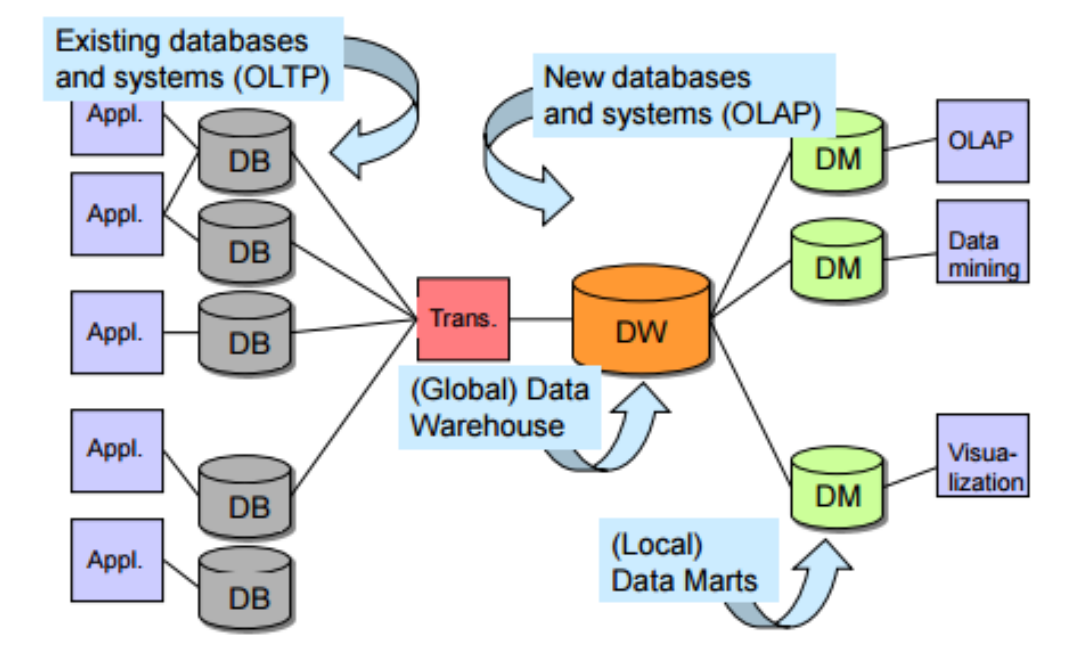
\includegraphics[width=.8\textwidth]{images/data_warehousing.png}
  \caption{Data Warehousing Structure}\label{fig:data_warehousing}
\end{figure}

DWs can have different structures.
One options is a \textbf{central DW} where all data is stored in one point.
This approach is very simple to manage but has bad performance due to the massive workload at that point.\\
A second variety is to have \textbf{multiple data marts} which are aimed at specific departments and store corresponding data.
The DW only exists logically.
This approach increases performance due to the distributed workload but is more complex.\\
The most complex but also most performant approach is to have a central warehouse where data is distributed to \textbf{data marts on multiple tiers}.
When querying, data is aggregated and reduced as it moves through tiers.\\

Data warehousing is a good approach to handle large amounts of data.
As always, it does not only have advantages though.
DW projects are usually very costly in time (12 - 36 month) and money (1 million US\$ or more).
Furthermore no design methodologies, insufficient training and some ethical considerations (security, privacy) exist.

